%\documentclass[titlepage]{jsarticle}

%\usepackage[dvipdfmx]{graphicx}

%数式用パッケージ
%\usepackage{amsmath, amssymb}
%\usepackage{mathtools}
%\usepackage{cancel}
%\usepackage{cases}
%\usepackage{bm}

%ファインマングラフ用パッケージ
%\usepackage{feynmf}

%ファインマンスラッシュ
%\newcommand{\Slash}[1]{{\ooalign{\hfil/\hfil\crcr\(#1\)}}}

%\title{課題研究P2\\J-PARC MLF  のミューオンビームを用いた\\ミューオン崩壊に関する諸量の測定}
%\author{阿部倫史,池満拓司,小田川高大,田島正規\\羽田野真友喜,早川龍,三野裕哉}
%\date{\today}

%\begin{document}

\section{序論}
本研究の目的はミューオンの崩壊現象を通して,標準模型,とくに弱い相互作用に関する各種の検証を行うことである.今回の実験で測定したい量は以下の三つである.

\begin{description}
\item[ミューオンの寿命]

ミューオンは弱い相互作用によって崩壊することが知られており,その寿命は標準模型によって計算されている.今回の実験ではミューオンビームを標的中で止めて,ミューオンの寿命を測定し.その値を理論値と比較して標準模型の検証を行う.
\item[ミッシェルパラメータ]

ミューオンの崩壊によって出てきた電子(陽電子)のエネルギースペクトルは,ミッシェルパラメータと呼ばれるいくつかのパラメータを用いて定式化でき,弱い相互作用の$V - A$ 理論ではこの値が決定されている.また,このエネルギースペクトルにはミューオンのスピンと陽電子の運動量がなす角$\theta$ についてその$\cos \theta$ に比例する特徴的な項が存在し,これは弱い相互作用のパリティ対称性の破れを表している.今回の実験ではこのエネルギースペクトルを求めることでミッシェルパラメータの値を決定し,弱い相互作用のパリティ対称性の破れを確認するとともに,$V - A$ 理論の妥当性を検証する.
\item[$g$ 因子]

ミューオンの$g$ 因子の測定は標準模型の検証に用いられる典型的な実験の一つであり,とくに現在,標準模型を超えた物理の存在をも示唆している可能性がある.今回の実験ではミューオンビームを止める標的中に磁場をかけることでミューオンを歳差運動させ,$g$ 因子の測定をめざす.
\end{description}

また,これらの実験を通して粒子ビームを用いた素粒子実験に触れ,その方法を会得することを目的とする.

\section{理論}
本節では今回の実験で測定する物理量についてその背景にある理論を概説する.なお,詳しい計算等については,一部は付録を見るか,あるいは参考文献を参照してほしい.以下,自然単位系($\hbar = c = 1$) を用いる.

\subsection{ミューオンとは}
ミューオン($\mu^{\pm}$)は1936年にAnderson らによって宇宙線から発見された,標準模型におけるレプトンの第二世代に属する素粒子である.$\mu^{\pm}$ は電子と同じ電荷$\pm e$,スピン$1/2$ を持ち,質量はその約$200$ 倍である.より正確には
	\[ m_{\mu} = 105.6583745 \pm 0.0000024~\mathrm{MeV}\]
と測定されている\cite{PDG}.
	
\subsection{ミューオンの寿命}
$\mu^{\pm}$ はほぼ100 \% の崩壊確率で次の崩壊を起こす\cite{PDG}.
\begin{eqnarray}
\mu^{-} \rightarrow e^{-} + \nu_{\mu} + \Bar{\nu}_{e}\\
\mu^{+} \rightarrow e^{+} + \Bar{\nu}_{\mu} + \nu_{\mu}
\label{eq:theory_muondecay}
\end{eqnarray}
今回の実験では$\mu^{+}$ を用いるので,以下$\mu^{+}$ についてその寿命を計算する.
	
\begin{figure}
\centering
\begin{fmffile}{feynmanzu1}
\begin{fmfgraph*}(120,80)

\fmfleft{mui}
\fmfright{numuo,eo,nueo}
				
\fmflabel{$\mu^{+}(p, r)$}{mui}
\fmflabel{$e^{+}(p', r')$}{eo}
\fmflabel{$\nu_e(q_{1}, r_{1})$}{nueo}
\fmflabel{$\bar{\nu}_{\mu}(q_{2}, r_{2})$}{numuo}
				
\fmf{fermion}{numuo,numumu,mui}
\fmf{boson,label=$W(k)$}{numumu,enue}
\fmf{fermion}{eo,enue}
\fmf{fermion}{enue,nueo}
				
\fmflabel{$\alpha$}{enue}
\fmflabel{$\!\!\!\beta$}{numumu}

\end{fmfgraph*}
\end{fmffile}
\vspace{10pt}
\caption{$\mu^{+}$ の崩壊のファインマン図.}
\label{zu:muondecay}
\end{figure}
	
$\mu^{+}$ の崩壊は図~\ref{zu:muondecay} のようなファインマン図で表される.標準模型(ワインバーグ=サラム理論)によればこの過程のファインマン振幅は
\begin{align}
\mathcal{M} = &-g_{W}^2\left[\Bar{u}(\bm{q_{1}})\gamma^{\alpha}(1 - \gamma_{5})v(\bm{p'})\right] \notag \\ 
&\times \frac{-(-g_{\alpha\beta} + k_{\alpha}k_{\beta}/m_{W}^2)}{k^{2} - m_{W}^2 + i\epsilon}\left[\Bar{v}(\bm{p})\gamma^{\beta}(1 - \gamma_5)v(\bm{q_{2}})\right]
\label{eq:theory_muondecayamp}
\end{align}
と書ける.ただし$p, q, k, \alpha, \beta$ などは図~\ref{zu:muondecay} に対応し,$g_{W}$ は弱い相互作用の結合定数である.その他の記法は付録A に記載している通りである.ここで,$m_{W}^2$ が$k^2$ にくらべて十分大きいとし,$m_{W} \rightarrow \infty$ の極限をとって計算すると,$V-A$ 理論の結果と一致する.この詳細な計算は付録A に掲載するが結果として$\mu^+$ の寿命
\begin{equation}
\tau_{\mu} = \frac{192\pi^3}{G^{2} m_{\mu}^{5}}
\label{eq:thory_muonlifetime}
\end{equation}
が得られる.ここで$G$ はFermi 結合定数である.

実際の測定値としては
\[\tau_{\mu} = 2.1969811 \pm 0.0000022 \times 10^{-6}~\mathrm{s}\]
という値が得られている\cite{PDG}.
	
\subsection{ミッシェルパラメータ}
式\eqref{eq:theory_muondecay} の$\mu^{+}$ 崩壊で出てくる$e^{+}$ を考える.静止した$\mu^{+}$ が崩壊する時,運動量とエネルギーの保存から$e^{+}$ が持ちうる最大エネルギーは$m_{\mu}/2 \simeq 50~\mathrm{MeV}$ であり,完全に偏極した$\mu^{+}$ の崩壊を静止系で考えると,出てくる$e^{+}$ のエネルギー及び角度分布はミッシェルパラメータと呼ばれる四つのパラメータ$\rho, \eta, \xi, \delta$ を用いて次のようにあらわすことができる\cite{michel_parameter}.
\begin{align}
\frac{d^2\Gamma}{x^{2}dxd(\cos \theta)} \propto& \,\,(3 - 3x) + \frac{2}{3}\rho (4x - 3) \notag \\
&+ 3 \eta \,x_{0} \frac{1-x}{x} + \xi \cos \theta \left[(1 - x) + \frac{2}{3} \delta (4x - 3)\right]
\label{eq:theory_michel}
\end{align}
ここでニュートリノの質量や輻射補正は無視した.ただし,$\theta$ は$e^{+}$ の運動量と$\mu^{+}$ のスピンのなす角度であり,$x$ は$e^{+}$ のエネルギーの最大値が1 となるように規格化したものである.また,$x_0$ は$e^{+}$ のエネルギーが$m_{e}$ のときの$x$ の値であり,これは通常無視できるので第3 項は考えないことも多い.

$\theta = \pi/2$ の位置で,もしくは全$\theta$にわたって測定した場合にはスピンに関係する第4項が0となるため,第1 項,第2 項のみを考えればよい.このとき式\eqref{eq:theory_michel} から
\begin{equation}
\frac{d\Gamma}{x^{2}dx} \propto (3 - 3x) + \frac{2}{3}\rho (4x - 3)
\label{eq:theory_michel2}
\end{equation}
となる.

Lorentz 共変な相互作用においては$\rho$ は $0, 0.75, 1$ のいずれかになることが分かっている\cite{michel_interaction}.入射粒子数で規格化すると,結局$\Gamma$ は$\rho$ によらないので式\eqref{eq:theory_michel2} をそのまま描いて,測定で得られるグラフの形は図\ref{zu:michelpar} のいずれかのようになる.
\begin{figure}[htbp]
\centering
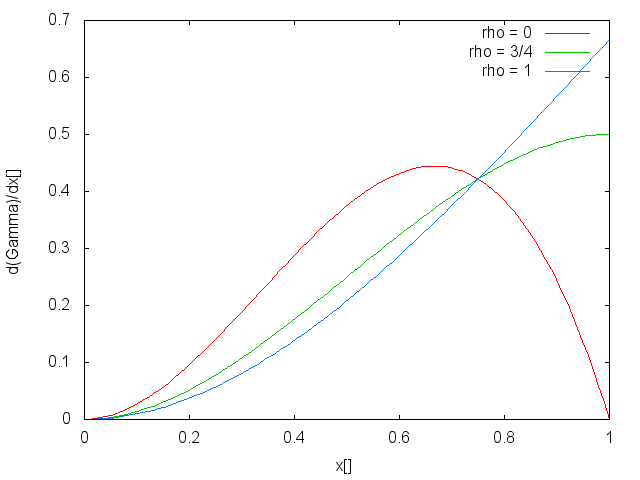
\includegraphics[width = 0.5\textwidth]{figure/abe/michelgraph.eps}
\caption{Michel 崩壊の各$\rho$ に対するスペクトル.Lorentz 共変な相互作用において許される$\rho$ の値についてそれぞれ描いた.}
\label{zu:michelpar}
\end{figure}
これらのグラフは大きく形が異なっているため,測定で得られたスペクトルを見ればある程度の相互作用の形を知ることができる.

特に,$V-A$ 理論では
\[ \rho = \xi\delta = \frac{3}{4},\, \eta = 0,\, \xi = 1 \]
となる.

また,実際には輻射補正を考えるとたとえば$\rho$ は$3 \sim 7$~\% ほど小さく測定されることが知られている.

現在のミッシェルパラメータの測定値は
\begin{align*}
\rho &= 0.74979 \pm 0.00026\\
\eta &= 0.057 \pm 0.034\\
\delta &= 0.75047 \pm 0.00034\\
\xi &= 1.0009^{+0.0016}_{-0.0007}
\end{align*}
である\cite{PDG}.
	
\subsection{ミューオンの$g$因子}

ミューオンの$g$ 因子は
\begin{equation}
\mu_\mu= g \cdot \frac{e\hbar}{2m_{\mu}c} \cdot \frac{S}{\hbar}
\end{equation}
で定義される無次元量である.

$\mu^{+}$ を含む,ディラック場で表されるようなフェルミ粒子の運動は次のDirac 方程式で記述される.
\begin{equation}
(i\Slash{\partial} - m)\psi(x) = 0
\label{eq:theory_dirac}
\end{equation}
ここで記法は付録A と同じとする.

次に式\eqref{eq:theory_dirac} をもとにして外場としての電磁場$A_{\mu}$ が存在する状態での方程式を考える.U(1) 局所ゲージ対称性を課すと,共変微分$D_{\mu} = \partial_{\mu} + ieA_{\mu}$ を定義できて,
\begin{equation}
(i\Slash{D} - m)\psi(x) = 0
\label{eq:theory_diracwitha}
\end{equation}
となる.

ここから非相対論的近似を行うために,いままで用いてきた自然単位系$\hbar = c = 1$ から$\hbar$ と$c$ を復活させる.$A_{\mu} = (\phi, \bm{A})$ とおくと,
\begin{equation}
i\hbar\frac{\partial}{\partial t}\psi(x) = \left\{c\bm{\alpha}\cdot (\bm{p} - e\bm{A}) + \beta m c^{2} + e \phi\right\}\psi(x)
\label{eq:theory_diracwithaphi}
\end{equation}
となる.スピノル$\psi(x)$ を
\begin{equation}
\psi(x) = \begin{pmatrix}
\chi_{1} (x)\\
\chi_{2} (x)
\end{pmatrix} \exp \left( - i \frac{mc^{2}}{\hbar} t\right)
\end{equation}
と書き,式\eqref{eq:theory_diracwithaphi} に代入すると
\begin{align}
i\hbar\left( -i\frac{mc^{2}}{\hbar} + \frac{\partial}{\partial t}\right) \chi_{1} = c\bm{\sigma}\cdot(\bm{p} - e \bm{A})\chi_{2} + (mc^{2} + e\phi)\chi_{1} \label{eq:theory_chi1}\\ 
i\hbar\left( -i\frac{mc^{2}}{\hbar} + \frac{\partial}{\partial t}\right) \chi_{2} = c\bm{\sigma}\cdot(\bm{p} - e \bm{A})\chi_{1} - (mc^{2} - e\phi)\chi_{2} \label{eq:theory_chi2}
\end{align}

非相対論近似においては式\eqref{eq:theory_chi2} について時間微分項が無視でき,またスカラーポテンシャルによるエネルギーも無視できるので
\begin{equation}
\chi_{2} = \frac{1}{2mc}\bm{\sigma}\cdot(\bm{p} - e\bm{A})\chi_{1}
\end{equation}
となる.これを式\eqref{eq:theory_chi1} に代入し,$\sigma$ 行列に関する計算を行えば
\begin{equation}
i\hbar\frac{\partial}{\partial t}\chi_{1} = \left\{\frac{(\bm{p} - e\bm{A})^{2}}{2m} + e\phi - \frac{e\hbar\bm{\sigma}}{2m}\cdot\bm{B}\right\}\chi_{1}
\label{eq:theory_pauli}
\end{equation}
という,Pauli 方程式が得られる.ここで$\bm{B} = \nabla \times \bm{A}$ であり,磁束密度を表す.式\eqref{eq:theory_pauli} よりスピン$\hbar\bm{\sigma}/2$ がもつ磁気モーメントは軌道角運動量の場合の二倍であり,この場合$g$ 因子は2 であることがわかる.

上のような計算を行えばDirac 方程式からミューオンの$g$ 因子は2 と求まる.QED (量子電磁力学)による考察を行うと,$g$ 因子には補正がかかることが分かっている.この$g$ 因子の2 からのずれを異常磁気能率 (anomalous magnetic moment) と呼ぶ.例えば二次の摂動において異常磁気能率に寄与する過程は図\ref{zu:vertexcorr} で表される過程である\cite{schwinger}.

\begin{figure}[h]
\centering
\begin{fmffile}{feynmanzu2}
\begin{fmfgraph*}(100,80)
				
\fmfleft{mui}
\fmfright{muo}
\fmfbottom{ai}
				
\fmflabel{$\mu$}{mui}
\fmflabel{$\mu$}{muo}
\fmflabel{$\gamma$}{ai}
				
\fmf{fermion}{mui,muig,muia}
\fmf{boson}{ai,muia}
\fmf{boson,left=0.5,tension=0.2}{muig,muog}
\fmf{fermion}{muia,muog,muo}
				
\end{fmfgraph*}
\end{fmffile}
\vspace{10pt}
\caption{二次の摂動における異常磁気能率への寄与過程.}
\label{zu:vertexcorr}
\end{figure}

図~\ref{zu:vertexcorr} で表される過程の寄与は$\alpha/2\pi$ (ここで$\alpha$ は微細構造定数$1/137$)である.

このような寄与をQED のより高次の摂動についても考えることができ,また一方でQED のレプトニックな過程以外の$W, Z$ ボソンを含む電弱理論に関して,あるいはハドロンが関与する過程に関しても考えることができる.このようにして,さまざまな相互作用を加味した異常磁気能率の理論値は
\[a_{\mu} = (g -2)/2 = 116591804(51) \times 10^{-11}\]
であり,その測定値は
\[a_{\mu} = 116592089(63) \times 10^{-11}\]
である\cite{g-2_theory, g-2_experiment}.
これらはQED の正しさを証明する一方で,標準模型の理論値とも$3\sigma$ 以上の有意な差があり,ここに新たな物理があることが期待されている.実際,未発見の粒子が存在して上に述べたような過程の他にその粒子の寄与を考えると,計算するべきファインマン図が増え,その分異常磁気能率に対する計算値も変わることになる.

$g$ 因子の測定は新しい物理の探索を目的として現在の素粒子物理学実験においてもっとも精密な計算と測定が行われている例である.

\section{実験原理}
本節では今回の実験の原理について説明する.今回の実験ではミューオン ($\mu^{+}$) ビームを用いてミューオンの崩壊寿命,ミッシェルパラメータ,そして$g$ 因子を測定する.そのために用いる検出器としてNaI (Tl) シンチレータとプラスチックシンチレータを採用する.なお,ミューオンビームの詳細は次節に含めている.

\subsection{寿命測定の原理}
ミューオンビームは標的で止められる.静止したミューオンは式\eqref{eq:thory_muonlifetime}の寿命$(\tau_\mu)$ を持つため,
\begin{equation}
\frac{dN_\mu}{dt} = -\frac{1}{\tau_\mu} N_{\mu}
\end{equation}
に従い崩壊し,この際にミューオンはほぼ100~\% の確率で陽電子を一つ出す.崩壊して出てくる陽電子の数は崩壊したミューオンの数と一致し
\begin{equation}
\frac{dN}{dt} = N_0 \exp{\left(-\frac{t}{\tau_\mu}\right) }
\end{equation}
で減少する.つまり陽電子を検出し,計数の時間変化を指数関数でフィッティングすれば寿命を求めることができる.

\subsection{ミッシェルパラメータ測定の原理}
今回はミッシェルパラメータのうち$\rho$ を測定するための実験を行なった.理論の節で述べたように$\rho$ の測定にはミュオンのスピンの向きに対して,$\theta = \pi / 2$ の位置で観測,または無偏極のミューオンが崩壊した時の$e^{+}$ のエネルギー分布を測定しなくてはならない.

ミューオンビームは進行方向にスピン偏極しているため,標的からビーム方向に対して$90^{\circ}$ の向きに検出器を設置してエネルギーを測定,得られたエネルギースペクトルを式\eqref{eq:theory_michel2} でフィッティングすれば,$\rho$ を求めることができる.この際,最大50~MeVの陽電子が出るので,50~MeV陽電子を止められるような検出器が要求される.また実際には,$90^{\circ}$ 方向に検出器を置くことが困難だったことやデータ量の関係から,後述する$g$ 因子測定のデータを利用して,全スピン方向で積分した無偏極ミューオンとして$\rho$ を求めた.また,この解析によりスピン部分のデータが得られたため,最終的にはミッシェルパラメータの$\xi,\;\delta$ の解析も行った.

\subsection{$g$ 因子測定の原理}
ミュオンのスピンは磁場中で歳差運動をする.一様磁場中において,磁場方向を$z$軸とすると,磁場とスピンの相互作用のハミルトニアンは,
\begin{equation}
\hat{H} = - g \frac{e}{2m_\mu} \hat {\textsl{\textbf {S}}} \cdot \textsl{\textbf {B}} = - g \frac{e}{2m_\mu}  \hat{S_z} B
\end{equation} 
であるので,Heisenberg方程式より,
\begin{equation}
\frac{d\hat{S_x}}{dt} =  g \frac{eB}{2m_\mu}\hat{S_y} 
\end{equation} 
\begin{equation}
\frac{d\hat{S_y}}{dt} = - g \frac{eB}{2m_\mu}\hat{S_x} 
\end{equation} 
\begin{equation}
\frac{d\hat{S_z}}{dt} = 0 
\end{equation} 
を得る.スピン初期状態を
\begin{equation}
\langle \textsl{\textbf {S}}(t=0)\rangle = (C,0,0)
\end{equation} 
とすれば,
\begin{equation}
\langle S_x \rangle= C\cos{(g\frac{eB}{2m_\mu}t)}
\end{equation}
\begin{equation}
\langle S_y \rangle= -C\sin{(g\frac{eB}{2m_\mu}t)}
\end{equation}
とスピンが$xy$平面内で回転することがわかり,その角速度$\omega$は,
\begin{equation}
\omega = g\frac{eB}{2m_\mu}
\end{equation}
となる.式\eqref{eq:theory_michel} の通り陽電子はミューオンのスピンの方向に出やすいので,磁場を通した標的でミューオンビームを止めると,陽電子の計数は指数的な減少に周期$2\pi / \omega$ の振動が加わったものになる.よってその周期から$g$ 因子を求めることができる.

%\end{document}
